\documentclass[11pt]{amsart}
\usepackage[T1]{fontenc}
\usepackage{newtxtext,newtxmath}
\usepackage{microtype}
\usepackage{booktabs}
\usepackage{tikz}
\usepackage[hidelinks]{hyperref}
\usepackage[letterpaper,textwidth=6.5in,textheight=9in]{geometry}

\newtheorem{theorem}{Theorem}[section]
\newtheorem{lemma}[theorem]{Lemma}
\newtheorem{proposition}[theorem]{Proposition}
\newtheorem{corollary}[theorem]{Corollary}
\theoremstyle{definition}
\newtheorem{definition}[theorem]{Definition}
\theoremstyle{remark}
\newtheorem{remark}[theorem]{Remark}
\numberwithin{equation}{section}
\newcommand{\R}{\mathbb R}
\newcommand{\norm}[1]{\lVert #1\rVert}
\newcommand{\abs}[1]{\lvert #1\rvert}
\newcommand{\rhoopt}{\rho_*}
\newcommand{\Ropt}{R_*}
\newcommand{\pil}{\pi_{\mathrm{lo}}}
\newcommand{\piu}{\pi_{\mathrm{up}}}
\newcommand{\rhol}{\rho_{\mathrm{lo}}}
\newcommand{\rhou}{\rho_{\mathrm{up}}}

\title[Fifteen equal circles in a circle]{Packing fifteen equal circles in a circle}
\author{Grant Huffman}
\email{huffma97@purdue.edu}
\date{October 6, 2026}
\subjclass[2020]{Primary 52C15}
\keywords{Circle packing, fifteen circles, exact arithmetic, computer-assisted proof, interval certificates}
\thanks{Prepared with AI assistance from OpenAI Codex. The accompanying single-file Lean formalization has passed compilation and an axiom audit. Two exhaustive finite checks use compiled evaluation. Independent review is invited.}

\begin{document}
\begin{abstract}
I present a computer-assisted proof that the smallest circular container for
fifteen unit-radius disks has radius
\[
 \Ropt=1+\sqrt{6+\frac{2}{\sqrt5}+4\sqrt{1+\frac{2}{\sqrt5}}}.
\]
The attaining arrangement is classical. The lower bound covers arbitrary
placements, without assuming symmetry or a prescribed contact graph.
A smaller packing would give fifteen points separated strictly by more than
two in a fixed disk. Maximizing the number of boundary points places every
remaining point inside a smaller disk and reduces the problem to 1,139
circular orders. Exact rational certificates exclude all radial boxes except
neighborhoods of the sharp arrangement. In those neighborhoods a coercive
inequality on an odd five-cycle forces equality and rules out strict
separation. Two independently implemented arithmetic verifiers accept every
certificate. A single Lean file proves the least-radius statement using the
original Formal Conjectures packing definitions. The geometric argument,
local exclusion and checker soundness are kernel-checked; acceptance of the
saved forest and coverage of all binary words use Lean's compiled evaluator.
The proof and computational artifacts are provided for independent review.
\end{abstract}
\maketitle

\section{Introduction}

The problem of packing congruent disks into a circular container has a long
history. Kravitz~\cite{kravitz} gave small packings, and Pirl~\cite{pirl}
proved optimality for several small cases. The fifteen-disk arrangement
considered here appears in the survey of Graham, Lubachevsky, Nurmela and
\"Osterg\aa rd~\cite{graham}. Ekanayake and LaFountain~\cite{ekanayake}
give an independent proof for fourteen disks and describe the previously
proved cases as $N\leq14$ and $N=19$. The fifteen-disk case is also stated as
an open problem in Google DeepMind's Formal Conjectures
repository~\cite{formalconjectures}.

For $R\geq0$ let
\[
 B_R=\{x\in\R^2:\norm{x}<R\},\qquad B=B_1.
\]
A packing consists of fifteen images of $B$ under Euclidean isometries,
pairwise disjoint and contained in $B_R$. These sets are open: tangencies
between unit disks, and tangencies with the container, are permitted.

\begin{theorem}\label{thm:main}
The least radius of a circular container admitting such a packing is
\begin{equation}\label{eq:radius}
 \Ropt=1+\sqrt{6+\frac{2}{\sqrt5}+4\sqrt{1+\frac{2}{\sqrt5}}}
       =4.52135696470616424090\ldots.
\end{equation}
The lower-bound assertion includes all placements of the fifteen disks.
\end{theorem}

The proof has three parts. I first give the attaining construction and
reduce a hypothetical smaller packing to a strict point-separation problem.
I then normalize a strict counterexample by maximizing its integer number
of boundary points. Finally I exclude every normalized configuration by a
finite family of exact certificates and a local analytic lemma. The
certificates have 154,291 nodes and can be checked with the Python standard
library alone. The certificate search is not part of the logical argument:
only the saved witnesses and their exact verification are used.

\section{Centers and the attaining construction}

\begin{lemma}\label{lem:centers}
Two open unit disks centered at $x,y$ are disjoint if and only if
$\norm{x-y}\geq2$. The disk centered at $x$ is contained in $B_R$ if and
only if $\norm{x}+1\leq R$.
\end{lemma}
\begin{proof}
If $\norm{x-y}<2$, their midpoint belongs to both disks. Conversely, a common
point would contradict the triangle inequality when $\norm{x-y}\geq2$.
The inequality $\norm{x}+1\leq R$ implies containment because every vector
$v$ with $\norm{v}<1$ satisfies $\norm{x+v}<\norm{x}+1$. If
$\norm{x}+1>R$, a vector of norm sufficiently close to one pointing outward
from $x$ produces a point outside the container. At $x=0$, any unit
direction has the same effect.
\end{proof}

Thus the container radius is one plus the least radius needed for fifteen
centers with pairwise distances at least two. Put
\begin{equation}\label{eq:constants}
 h=\frac\pi5,\quad
 a=\csc h=\sqrt{2+\frac2{\sqrt5}},\quad
 u=\cot h=\sqrt{1+\frac2{\sqrt5}},\quad
 \rhoopt=\sqrt{(u+2)^2+1},\quad
 \alpha=\arcsin\frac1{\rhoopt}.
\end{equation}
In particular $\Ropt=1+\rhoopt$.

Take a regular pentagon with inner centers
\[
 I_k=a(\cos(2kh),\sin(2kh)),\qquad 0\leq k<5,
\]
and use cyclic indices. Its side $I_kI_{k+1}$ has outward unit normal
\[
 n_k=(\cos((2k+1)h),\sin((2k+1)h)).
\]
The ten other centers are
\begin{equation}\label{eq:outer}
 O_k^-=I_k+2n_k,\qquad O_k^+=I_{k+1}+2n_k.
\end{equation}
In coordinates in which $n_k$ is horizontal, the two inner endpoints are
$(u,-1),(u,1)$ and the two outer endpoints are $(u+2,-1),(u+2,1)$.
Every outer center therefore has norm $\rhoopt$. An inner side, an outer
pair on the same side, and the displacement from an inner endpoint to its
corresponding outer center all have length two.

The outer angles are $(2k+1)h\pm\alpha$. Their consecutive gaps alternate
between $2\alpha$ and $2(h-\alpha)$. I have $\alpha<h/2$, since
$\rhoopt>3.52>1+\sqrt5=\csc(h/2)$. Hence their least minor angular
separation is $2\alpha$, and every outer pair has distance at least
$2\rhoopt\sin\alpha=2$. The inner pentagon diagonals exceed its sides.
The nearest inner ray to an outer center is its source endpoint, at angular
distance $h-\alpha$, where the distance is two. For fixed nonnegative
radii, the chord distance is nondecreasing with the minor central angle.
All inner--outer distances are therefore at least two. Lemma~\ref{lem:centers}
proves attainment of~\eqref{eq:radius}.

\begin{figure}[ht]
\centering
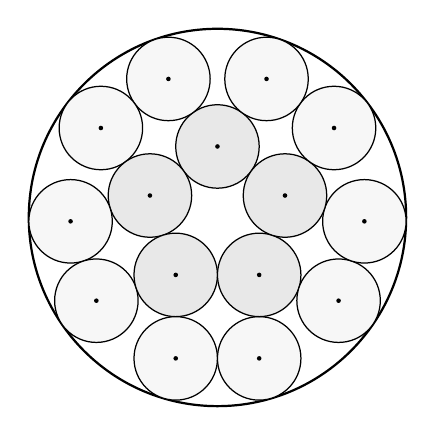
\begin{tikzpicture}[scale=.53]
 \pgfmathsetmacro{\aa}{sqrt(2+2/sqrt(5))}
 \pgfmathsetmacro{\uu}{sqrt(1+2/sqrt(5))}
 \pgfmathsetmacro{\rr}{1+sqrt((\uu+2)^2+1)}
 \draw[line width=.8pt] (0,0) circle (\rr);
 \foreach \k in {0,...,4}{
  \pgfmathsetmacro{\ang}{72*\k+90}
  \pgfmathsetmacro{\nextang}{72*(\k+1)+90}
  \pgfmathsetmacro{\normal}{72*\k+36+90}
  \pgfmathsetmacro{\ix}{\aa*cos(\ang)}
  \pgfmathsetmacro{\iy}{\aa*sin(\ang)}
  \pgfmathsetmacro{\jx}{\aa*cos(\nextang)}
  \pgfmathsetmacro{\jy}{\aa*sin(\nextang)}
  \pgfmathsetmacro{\ox}{\ix+2*cos(\normal)}
  \pgfmathsetmacro{\oy}{\iy+2*sin(\normal)}
  \pgfmathsetmacro{\px}{\jx+2*cos(\normal)}
  \pgfmathsetmacro{\py}{\jy+2*sin(\normal)}
  \draw[fill=black!9,line width=.45pt] (\ix,\iy) circle (1);
  \draw[fill=black!3,line width=.45pt] (\ox,\oy) circle (1);
  \draw[fill=black!3,line width=.45pt] (\px,\py) circle (1);
  \fill (\ix,\iy) circle (.055);
  \fill (\ox,\oy) circle (.055);
  \fill (\px,\py) circle (.055);
 }
\end{tikzpicture}
\caption{The classical attaining arrangement. Five centers form a regular
pentagon; ten centers lie on the outer circle. The proof of the lower bound
does not assume this structure.}
\label{fig:packing}
\end{figure}

\begin{lemma}\label{lem:strict}
If a packing exists in a container of radius less than $\Ropt$, then there
are fifteen points $x_i$ with $\norm{x_i}\leq\rhoopt$ and
$\norm{x_i-x_j}>2$ whenever $i\ne j$.
\end{lemma}
\begin{proof}
By Lemma~\ref{lem:centers}, its center radius $\rho_0$ is less than
$\rhoopt$. It is positive, since fifteen points with separation at least
two cannot all be zero. Multiplication of all centers by
$\rhoopt/\rho_0>1$ proves the assertion.
\end{proof}

It suffices to exclude this strict configuration at the fixed radius
$\rhoopt$. The non-strict attaining arrangement remains admissible.

\section{A maximal-boundary normalization}

Set
\begin{equation}\label{eq:D}
 D=\rhoopt-\frac4{\rhoopt}.
\end{equation}
\begin{proposition}\label{prop:normalize}
If a strict configuration from Lemma~\ref{lem:strict} exists, then one exists
with $m$ boundary centers, $1\leq m\leq10$, and with each of its $15-m$
remaining centers of norm less than $D$.
\end{proposition}
\begin{proof}
Choose a strict configuration for which the number $m$ of centers of norm
$\rhoopt$ is maximal. This maximum is attained because the set of attained
integers is a nonempty subset of $\{0,\ldots,15\}$. No compactness argument
or existence theorem for an optimal packing is required.

If $m=0$, choose a farthest center $x=sv$ with $\norm{v}=1$. Here $s>0$.
Replace $sv$ by $\rhoopt v$. For any other center $z$, $\norm{z}\leq s$ and
\begin{align}\label{eq:move}
 \norm{\rhoopt v-z}^2-\norm{sv-z}^2
 &= (\rhoopt-s)(\rhoopt+s-2\langle v,z\rangle)\\
 &\geq (\rhoopt-s)^2>0.\notag
\end{align}
This preserves strict separation and increases $m$, a contradiction.

Suppose now that an interior center of largest interior radius is $sv$,
with $D\leq s<\rhoopt$. Formula~\eqref{eq:move} preserves its distances
from all other interior centers. For a boundary center $\rhoopt w$, its
previous separation gives
\[
 \langle v,w\rangle<C(s),\qquad
 C(s)=\frac{\rhoopt^2+s^2-4}{2\rhoopt s}.
\]
The factorization
\begin{equation}\label{eq:factor}
 C(s)-C(\rhoopt)=
 \frac{(s-\rhoopt)(s-D)}{2\rhoopt s}\leq0
\end{equation}
shows that $\langle v,w\rangle<1-2/\rhoopt^2$. Consequently
$\norm{\rhoopt v-\rhoopt w}>2$ after replacement. Again $m$ increases,
contradicting its maximality. Every interior radius is thus less than $D$.

For the upper bound on $m$, consecutive boundary centers have angular gaps
greater than $2\alpha$. For $0<t<1$,
\begin{equation}\label{eq:asin}
 \arcsin t\geq t+\frac{t^3}{6}.
\end{equation}
Indeed, integrate $(1-t^2)^{-1/2}\geq1+t^2/2$, which follows by squaring
positive quantities. The rational bounds in Section~\ref{sec:constants}
give
\[
 11\left(\frac1{\rhoopt}+\frac1{6\rhoopt^3}\right)>\pi.
\]
Eleven boundary centers would therefore require total angular support
greater than $2\pi$. Any larger boundary set contains eleven such centers.
Hence $m\leq10$.
\end{proof}

The replacement in this proof is direct. Feasibility of a continuous path
between the old and new locations is unnecessary.

\section{Circular orders and exhaustive radial subdivision}

Write a boundary center as a zero and an interior center as a one, in
nondecreasing polar-angle order. A center at the origin may receive any
polar angle. Tied angles are allowed. Cyclic relabeling and reversal preserve
feasibility. Angles can be lifted to a closed window of length $2\pi$;
allowing both endpoints also handles a cyclic cut within a tied group.

For a binary word $b$ of length fifteen, let $\operatorname{can}(b)$ be the
lexicographically least word among its rotations and the rotations of its
reversal. Proposition~\ref{prop:normalize} leaves $k=15-m\in\{5,\ldots,14\}$
ones. Exhaustive enumeration gives the following representatives.
\begin{table}[ht]
\centering
\caption{All circular orders, modulo rotation and reversal.}
\begin{tabular}{@{}rrrrrrrrrrr@{}}
\toprule
$k$&5&6&7&8&9&10&11&12&13&14\\
Orders&111&185&232&232&185&111&56&19&7&1\\
\bottomrule
\end{tabular}
\label{tab:orders}
\end{table}
The total is 1,139. Coverage is established by enumerating the words, not
by assuming the numerical count in the table. The second verifier instead
enumerates all $2^{15}$ bit masks and compares sets of representatives.

All terminating decimals below denote exact rationals. Define
\begin{align}\label{eq:intervals}
 \rhol&=3.52135696470616424090,&
 \rhou&=3.52135696470616424092,\\
 D_{\mathrm{up}}&=\rhou-4/\rhou.\notag
\end{align}
The algebraic calculations in Section~\ref{sec:constants} prove
$\rhol<\rhoopt<\rhou$. Since $r-4/r$ is increasing for $r>0$, I also
have $D<D_{\mathrm{up}}$.

For each circular order, the root radial box assigns the interval
$[\rhol,\rhou]$ to every boundary variable and $[0,D_{\mathrm{up}}]$ to
every interior variable. These intervals are conservative relaxations.
The boundary centers of the geometric configuration all still have the
same actual radius $\rhoopt$.

If $r_i,r_j$ are interior radii, strict separation implies $r_i+r_j>2$.
An upper bound $H_j$ on $r_j$ therefore permits the conservative update
\begin{equation}\label{eq:propagate}
 L_i\gets\max\left(L_i,\ 2-\min_{j\ne i,\ b_j=1}H_j\right).
\end{equation}
A box with some $L_i>H_i$ is impossible. Otherwise an internal certificate
node selects an interior coordinate and divides its interval at its exact
rational midpoint. Both closed halves are retained. Thus every feasible
radius vector stays in at least one child, including a vector on a
subdivision boundary.

Every tree is finite. Its terminal boxes are excluded either by an angular
cycle, as in the next section, or by the analytic lemma of
Section~\ref{sec:local}. No heuristic pruning rule is accepted by a verifier.

\section{Exact angular-cycle certificates}\label{sec:cycles}

\begin{lemma}\label{lem:corner}
Let $r\in[L_1,H_1]$, $s\in[L_2,H_2]$, with nonnegative endpoints, and let
$0<t<\pi$. Suppose a rational $C_0\leq\cos t$ satisfies
\begin{equation}\label{eq:corner}
 (r-s)^2+2rs(1-C_0)\leq4
\end{equation}
at the four corners of the radial rectangle. Any two points of radii $r,s$
separated by more than two have minor central angle greater than $t$.
\end{lemma}
\begin{proof}
The left side of~\eqref{eq:corner} is separately convex in $r$ and $s$.
Its maximum on the rectangle is therefore attained at a corner. The squared
chord at angle $t$ is bounded above by this expression. Chord distance is
nondecreasing with the minor angle on $[0,\pi]$, so strict separation
requires an angle greater than $t$. If one radius is zero, the same corner
bound makes the distance at most two, already excluding strict separation;
no division by a radius is used.
\end{proof}

Let $\phi_0\leq\cdots\leq\phi_{14}$ lie in a window of length $2\pi$.
A certified minor-angle lower bound $t_{ij}\geq0$ implies
\begin{equation}\label{eq:edge}
 \phi_j-\phi_i+2\pi\,\boldsymbol1_{i>j}\geq t_{ij}.
\end{equation}
For $t_{ij}=0$ this is automatic. For $t_{ij}>0$, both directed angular
separations are at least the minor-angle bound.

Consider a directed simple cycle $i_0,i_1,\ldots,i_{q-1},i_q=i_0$, and
write $w=\#\{\ell:i_\ell>i_{\ell+1}\}$. Summing~\eqref{eq:edge} cancels
the angle variables and gives
\begin{equation}\label{eq:cycle}
 \sum_{\ell=0}^{q-1}t_{i_\ell i_{\ell+1}}\leq2\pi w.
\end{equation}
Put
\begin{equation}\label{eq:piinterval}
 \pil=3.14159265358979323846,\qquad
 \piu=3.14159265358979323847.
\end{equation}
Since $\pi<\piu$, a certificate with sum greater than $2\piu w$ contradicts
\eqref{eq:cycle}.

The saved bounds have the form $t=n/2^{40}$, where $n$ is a nonnegative
integer. Each positive bound is checked to be less than $\pil$. The first
verifier uses
\begin{equation}\label{eq:cosine}
 P(t)=\sum_{j=0}^{21}\frac{(-1)^j t^{2j}}{(2j)!}\leq\cos t.
\end{equation}
The first omitted term is positive, and the successive omitted terms
decrease in magnitude for $0\leq t\leq\pi$. The alternating-series
remainder proves~\eqref{eq:cosine}. On scale $S=2^{192}$, the verifier
rounds each positive term down and each negative term's magnitude up.
If the resulting integer is $K$, then $K/S\leq P(t)\leq\cos t$.
It checks~\eqref{eq:corner} with $C_0=K/S$ using integer and rational
arithmetic only.

The independent verifier uses a different polynomial:
\begin{equation}\label{eq:sine}
 T(z)=\sum_{j=0}^{20}\frac{(-1)^j z^{2j+1}}{(2j+1)!}
       \geq\sin z\geq0,\qquad 0\leq z\leq\pi/2.
\end{equation}
It verifies at all four corners
\[
 (r-s)^2+4rs\,T(t/2)^2\leq4.
\]
This bounds the squared chord because
$1-\cos t=2\sin^2(t/2)$. It imports neither the first verifier's arithmetic
module nor a numerical optimization package.

\section{The sharp local configuration}\label{sec:local}

Finite subdivision must account for neighborhoods of the attaining
configuration, where an exclusion with a fixed positive margin is
impossible. The following lemma supplies that step.

\begin{lemma}[Odd-cycle coercivity]\label{lem:local}
Suppose five interior centers alternate, in circular order, with pairs of
boundary centers of radius $\rhoopt$. If every interior radius $r_i$ satisfies
$\abs{r_i-a}\leq\delta=1/100$ and every pair of centers is at distance at
least two, then $r_i=a$ for all $i$. In particular this neighborhood contains
no strict configuration.
\end{lemma}
\begin{proof}
On this neighborhood define
\[
 b(r)=\arccos\frac{\rhoopt^2+r^2-4}{2\rhoopt r},\qquad
 c(r,s)=\arccos\frac{r^2+s^2-4}{2rs}.
\]
The arguments of $\arccos$ lie strictly between $-1$ and $1$ by the bounds
in Appendix~\ref{app:derivatives}. Let $g_i$ be the forward angular gap
from interior center $i$ to interior center $i+1$, with indices modulo five.
The direct pair constraint and the three successive gaps through the two
intervening boundary centers give
\begin{equation}\label{eq:localgap}
 g_i\geq\max\{c(r_i,r_{i+1}),\ b(r_i)+2\alpha+b(r_{i+1})\},
 \qquad \sum_i g_i=2\pi.
\end{equation}
These inequalities use only the circular order, not equality of the radii.

At the reference point both quantities in the maximum equal $2h$:
$c(a,a)=2h$ and $b(a)+\alpha=h$. The second identity follows also from the
endpoint tangency in the construction~\eqref{eq:outer}. Put
\[
 x_i=r_i-a,\quad z_i=x_i+x_{i+1},\quad
 p=-\frac2{a^3\sin(2h)},\quad q=\frac ua=\cos h.
\]
Appendix~\ref{app:derivatives} proves
\begin{equation}\label{eq:derivativebounds}
 p<-\frac25,\qquad |p|<.46,\qquad .80<q<.82.
\end{equation}
An elementary cosine estimate, with exact rational expansions of the
cosine arguments, gives
\begin{align*}
 c(r_i,r_{i+1})
 &\geq2h+pz_i-3(x_i^2+x_{i+1}^2),\\
 b(r_i)+2\alpha+b(r_{i+1})
 &\geq2h+qz_i-3(x_i^2+x_{i+1}^2).
\end{align*}
For $z_i\geq0$ use the second inequality, and for $z_i<0$ the first.
Equation~\eqref{eq:localgap} then implies
\begin{equation}\label{eq:coercivegap}
 g_i\geq2h+\frac25\abs{z_i}-3(x_i^2+x_{i+1}^2).
\end{equation}

The five-cycle is odd, so
\begin{equation}\label{eq:oddidentity}
 2x_i=z_i-z_{i+1}+z_{i+2}-z_{i+3}+z_{i+4}.
\end{equation}
Taking absolute values and summing yields
\[
 \sum_i\abs{x_i}\leq\frac52\sum_i\abs{z_i},\qquad
 \sum_i x_i^2\leq\frac{5\delta}{2}\sum_i\abs{z_i}.
\]
Sum~\eqref{eq:coercivegap} and use $5(2h)=2\pi$ to obtain
\[
 2\pi\geq2\pi+\left(\frac25-15\delta\right)\sum_i\abs{z_i}
       =2\pi+\frac14\sum_i\abs{z_i}.
\]
All $z_i$ vanish. Equation~\eqref{eq:oddidentity} forces all $x_i=0$.
Now $g_i\geq2h$ and $\sum_i g_i=2\pi$, so each $g_i=2h$. Adjacent inner
centers are consequently at distance exactly two. Strict separation is
impossible.
\end{proof}

An analytic leaf is accepted only for the word $(1,0,0)^5$, up to the
canonical convention, and only if all five entire interior intervals lie in
\begin{equation}\label{eq:localinterval}
 [a_{\mathrm{up}}-\delta,\ a_{\mathrm{lo}}+\delta],
 \qquad a_{\mathrm{lo}}\leq a\leq a_{\mathrm{up}}.
\end{equation}
This places every actual radius within $\delta$ of $a$. The actual boundary
radii still equal $\rhoopt$, so the exact common-radius hypothesis of
Lemma~\ref{lem:local} holds despite the relaxed boundary intervals elsewhere
in the computation.

\section{Exact constants and certificate verification}\label{sec:constants}

Every algebraic enclosure is computed using integer square roots. For
$x>0$ rational and $Q$ a positive integer, set
\[
 n=\left\lfloor\sqrt{\lfloor xQ^2\rfloor}\right\rfloor.
\]
Then $(n/Q)^2\leq x<((n+1)/Q)^2$. Apply this rule successively to $5$,
$1+2/\sqrt5$, $2+2/\sqrt5$ and the expression for $\rhoopt$, using
monotonicity of positive square roots and of reciprocal bounds. The two
verifiers use $Q=10^{50}$ and $Q=10^{45}$, respectively. Both prove all
enclosures in~\eqref{eq:intervals} and~\eqref{eq:localinterval}.

For $\pi$, use Machin's identity
\begin{equation}\label{eq:machin}
 \pi=16\arctan(1/5)-4\arctan(1/239).
\end{equation}
The tangent double-angle formula gives
$\tan(2\arctan(1/5))=5/12$ and
$\tan(4\arctan(1/5))=120/119$. Tangent subtraction therefore gives tangent
one for $4\arctan(1/5)-\arctan(1/239)$. This angle is positive and less
than $\pi/2$, proving~\eqref{eq:machin}. For an even number $M$ of terms,
\[
 A_M(d)=\sum_{j=0}^{M-1}\frac{(-1)^j}{(2j+1)d^{2j+1}}
\]
is a lower bound for $\arctan(1/d)$; adding the next positive term gives an
upper bound. Thirty terms in the first verifier, and twenty-eight in the
second, establish $\pil<\pi<\piu$. These bounds also prove the inequality
used in Proposition~\ref{prop:normalize} by the exact test
\[
 11\left(\frac1{\rhou}+\frac1{6\rhou^3}\right)>\piu.
\]

Each compressed certificate contains a complete binary tree. A subdivision
node records its coordinate and both children. A cycle leaf records its
ordered distinct indices and integer angle numerators. An analytic leaf
records its type; its order and radial neighborhood are checked from the
current box. Both verifiers reconstruct the box at every node, apply
\eqref{eq:propagate}, and reject invalid, repeated or unreachable nodes.
All nodes must be visited exactly once. Every circular order must occur
exactly once in the manifest, and every file's SHA-256 digest must match.

\begin{table}[ht]
\centering
\caption{The complete verification, with identical totals in both replays.}
\begin{tabular}{@{}lr@{}}
\toprule
Circular orders&1,139\\
Subdivision nodes&76,576\\
Angular-cycle leaves&77,490\\
Analytic-neighborhood leaves&225\\
Radial-contradiction leaves&0\\
Total tree nodes&154,291\\
Missing or unresolved orders&0\\
\bottomrule
\end{tabular}
\label{tab:verification}
\end{table}

The counts obey the forest identity
$77{,}715-76{,}576=1{,}139$. This identity is a consistency check, not a
replacement for the traversal and coverage checks. The latest standard
library replays completed in approximately 18.1 and 15.6 seconds on the
supplied host. Timing is not part of the mathematical proof.

\section{Completion of the lower bound}

\begin{proof}[Proof of Theorem~\ref{thm:main}]
Section 2 gives a packing at $\Ropt$. Suppose a smaller-radius packing
exists. Lemma~\ref{lem:strict} produces a strict configuration at center
radius $\rhoopt$. Proposition~\ref{prop:normalize} gives one with between
one and ten boundary centers, and all other centers of norm less than $D$.
Its circular order has a representative in Table~\ref{tab:orders}, and
its radii belong to that representative's root box.

Follow the certificate tree. Propagation preserves the actual radius vector;
each subdivision has a child containing it. A terminal box cannot have
inconsistent radial intervals. At a cycle leaf, Lemma~\ref{lem:corner}
and~\eqref{eq:cycle} contradict the exact recorded cycle sum. At an analytic
leaf, Lemma~\ref{lem:local} contradicts strict separation. Table~\ref{tab:verification}
and the complete replays establish that there are no other terminal cases
or unexamined circular orders. This contradiction excludes every smaller
radius. Together with attainment it proves the least-radius assertion.
\end{proof}

Fivefold symmetry is used in the attaining construction and is forced in
the local equality case. The global exclusion covers asymmetric
configurations and places no concentric-ring hypothesis on an arbitrary
packing.

\section{Reproducibility and formalization status}\label{sec:reproduce}

The companion archive \texttt{fifteen-circle-packing-proof-bundle.zip}
contains the full certificate forest, both verification programs, the
arithmetic module used by the first, their recorded outputs, and a detailed
proof report. Extract the archive and run, without Python's optimization
flag,
\begin{verbatim}
python verify_polar_certificates.py
python verify_polar_alternative.py
\end{verbatim}
Both programs must terminate normally with
\texttt{all\_cases\_verified=true}, 1,139 verified cases, and no missing
cases. Python 3.12 was used for the recorded replays. No package beyond the
standard library is needed. Assertions are part of the verification, so
\texttt{python -O} must not be used.

The generator used numerical calculations to propose witnesses and choose
subdivisions. None of those calculations is accepted as proof evidence.
The verifiers evaluate their mathematical tests with integers and exact
rationals. Their arithmetic checks establish the recorded inequalities;
the geometric interpretation, the analytic leaf and the exhaustive-coverage
argument are the mathematical obligations proved in the preceding sections.
Independent implementations provide a useful check on programming errors
but do not replace review of those obligations.

The exact formal target is
\texttt{SquarePacking.least\_fifteen\_circle\_packing\_in\_circle} in
\texttt{FormalConjectures/Wikipedia/SquarePacking.lean} at repository
commit \texttt{89294ea02bd7cd678d59984add52cb4baef3dbf4}. It asks for
\[
 \operatorname{IsLeast}
 \{R\in\R_{\geq0}:\text{a packing of fifteen unit disks in }B_R\text{ exists}\}
 \ \Ropt.
\]
Here the original Lean packing structure uses arbitrary isometric
equivalences of the Euclidean plane, pairwise disjoint images, and set
containment. Lemma~\ref{lem:centers} connects these definitions to the center
formulation. The accompanying single file
\texttt{FifteenCirclesInACircle.lean} proves the least-radius statement under
the name
\begin{verbatim}
FifteenCirclesInACircle.least_fifteen_circle_packing_in_circle
\end{verbatim}
The original conjecture's unspecified answer is filled with the radical
$\Ropt$; its admitted proof is not used. The file contains the construction,
normalization, polar ordering and symmetries, local analytic exclusion,
certificate decoder, checker soundness proofs, angle bounds, and all saved
certificate data. No companion certificate file is needed to compile it.

The final single file compiled successfully with Lean 4.33.1 and Mathlib
revision \texttt{0df444a360eaa60ab8c11dca51a86af692955474}, matching the
pinned Formal Conjectures project. A build receipt records the source
SHA-256 digest and compiler exit status. Lean accepts all 1,139 certificate
trees and checks every one of the $2^{15}=32{,}768$ binary radial words.
A proved enumeration lemma connects that finite list to arbitrary words,
and proved rotation and reflection lemmas connect each word to its saved
representative. Thus the final theorem includes the exhaustive-coverage
obligation as well as certificate acceptance and geometric soundness.

The formalization's trust boundary is explicit. The geometry, local lemma,
checker soundness, and 778 exact angle bounds are checked by the Lean
kernel. The two large finite acceptance checks use \texttt{native\_decide},
which trusts Lean's compiled evaluator. The final theorem's axiom audit
lists only \texttt{propext}, \texttt{Classical.choice}, \texttt{Quot.sound},
and the two generated native-evaluation axioms for forest acceptance and
word coverage. It contains no dependency on \texttt{sorryAx} or on an
assumed packing theorem. This is a formal computer-assisted proof with
compiled-evaluation trust; it is not a kernel-only replay of the two large
finite computations. The independent Python verifiers provide additional
reproducibility checks.

\section*{Acknowledgment of AI assistance}
OpenAI Codex assisted with the mathematical argument, exact certificate
generation and checking, manuscript preparation, and development of the
Lean formalization. Grant Huffman is the named author of this manuscript.
The mathematical claim and computational artifacts remain subject to
independent verification. No completed independent review is asserted.

\appendix
\section{Elementary bounds for the local lemma}\label{app:derivatives}

The exact algebraic enclosures imply
$1.701<a<1.702$ and $3.52<\rhoopt<3.53$. The neighborhood
$\abs{r-a},\abs{s-a}\leq1/100$ lies in $[1.69,1.72]^2$.
Write
\[
 C(r,s)=\frac{r^2+s^2-4}{2rs}.
\]
Put $r=a+x$, $s=a+y$, $z=x+y$, $S=x^2+y^2$, and $G=2/a^3$.
The exact identity
\begin{align*}
 2rs\bigl(C(r,s)-C(a,a)-Gz\bigr)
 &=S-2C(a,a)xy-2aGz^2-2Gxyz
\end{align*}
implies
\begin{equation}\label{eq:affinecos}
 C(r,s)\leq C(a,a)+Gz+2S.
\end{equation}
Indeed, $0<C(a,a)<.34$, $0<G<1$, $|z|\leq.02$,
$2|xy|\leq S$, and $rs>1$. The four terms on the right of the identity
are bounded above by $S$, $S$, $0$, and $.02S$, respectively.

For $B(r)=(\rhoopt^2+r^2-4)/(2\rhoopt r)$, set
$H=(a^2-\rhoopt^2+4)/(2\rhoopt a^2)$. A second exact identity gives
\[
 B(a+x)-B(a)-Hx
 =\frac{\rhoopt^2-4}{2\rhoopt a^2(a+x)}x^2\leq\tfrac12x^2.
\]
The coefficient bound follows from $3.52<\rhoopt<3.53$ and
$a,a+x\geq1.69$.

The reference geometry gives
\[
 \sin(2h)>.94,\qquad \sin b(a)=\frac2{a\rhoopt}>.33,
 \qquad -\sin(2h)p=G,\quad -\sin b(a)q=H.
\]
The exact algebraic enclosures imply $a^3<5$, $|p|<.46$, and
$.80<q=u/a<.82$, proving~\eqref{eq:derivativebounds}.
For $|x|,|y|\leq.01$, they also imply
\[
 (pz-3S)^2\leq S,\qquad (qx-3x^2)^2\leq\tfrac34x^2.
\]
For the first estimate, use $z^2\leq2S$, $S\leq.0002$, and
$(A-B)^2\leq2A^2+2B^2$. For the second, use
$|q-3x|\leq.85$.

Taylor's theorem for cosine alone, whose second derivative has absolute
value at most one, gives the global estimate
\[
 \cos(\theta+d)\geq\cos\theta-\sin\theta\,d-d^2/2.
\]
Apply this with $(\theta,d)=(2h,pz-3S)$ and
$(\theta,d)=(b(a),qx-3x^2)$. In the first case,
$3\sin(2h)S-d^2/2\geq2S$; in the second,
$3\sin b(a)x^2-d^2/2\geq x^2/2$. Combine these estimates with the
two exact cosine expansions. Monotonicity of $\arccos$ on its domain
proves the angular lower bounds used in Lemma~\ref{lem:local}.
The tested angles are less than $\pi$; if a tested angle is negative,
the corresponding lower bound follows from nonnegativity of $\arccos$.
These elementary inequalities are proved in the accompanying Lean
components without introducing inverse-trigonometric second derivatives.

\begin{thebibliography}{9}
\bibitem{ekanayake}
D. B. Ekanayake and D. J. LaFountain,
\emph{Tight partitions for packing circles in a circle},
Italian Journal of Pure and Applied Mathematics \textbf{51} (2024), 115--136.
\url{https://ijpam.uniud.it/online_issue/202451/10%20Ekanayake-LaFountain.pdf}.

\bibitem{graham}
R. L. Graham, B. D. Lubachevsky, K. J. Nurmela and P. R. J. \"Osterg\aa rd,
\emph{Dense packings of congruent circles in a circle},
Discrete Mathematics \textbf{181} (1998), 139--154.
\href{https://doi.org/10.1016/S0012-365X(97)00050-2}{doi:10.1016/S0012-365X(97)00050-2}.

\bibitem{formalconjectures}
Google DeepMind, \emph{Formal Conjectures},
\texttt{FormalConjectures/Wikipedia/SquarePacking.lean},
commit \texttt{89294ea02bd7cd678d59984add52cb4baef3dbf4}.
\url{https://github.com/google-deepmind/formal-conjectures}.
Accessed October 6, 2026.

\bibitem{kravitz}
S. Kravitz, \emph{Packing cylinders into cylindrical containers},
Mathematics Magazine \textbf{40} (1967), 65--71.

\bibitem{pirl}
U. Pirl, \emph{Der Mindestabstand von $n$ in der Einheitskreisscheibe
gelegenen Punkten}, Mathematische Nachrichten \textbf{40} (1969), 111--124.
\href{https://doi.org/10.1002/mana.19690400110}{doi:10.1002/mana.19690400110}.
\end{thebibliography}
\end{document}
